\documentclass[lineno,pdflatex,sn-basic,referee,]{sn-jnl}

\usepackage{amsmath}
\usepackage{amssymb}
\usepackage{booktabs}


% this fixes the line numbering
\makeatletter

\AtBeginDocument{\unsetvruler}
\makeatother

\usepackage[switch]{lineno}
\renewcommand\linenumberfont{\normalfont\tiny\sffamily}
\AtBeginDocument{\linenumbers}
\begin{document}
% end of line numbering fix

\title{A Method for Passive Identification of Spacecraft Using
Doppler-Based Trajectory Matching}

\author*[1]{\fnm{Fedor Ivanovich} \sur{Vtorov}}
\affil[1]{
  \orgdiv{Department of Automated Control Systems},
  \orgname{National University of Science and Technology MISIS},
  \city{Moscow},
  \country{Russia}
}

\abstract{
    This paper presents a passive method for identifying unknown spacecraft using the Doppler signature of a single satellite pass, requiring neither training data nor the precise knowledge of the transmitter carrier frequency. Doppler shifts are extracted from SDR IQ samples via a phase-locked loop and averaged into a one second time series. Candidates from an open Two-Line Element catalog are processed by a seven-stage filtering algorithm before predicted Doppler trajectories are generated using a computationally efficient combination of SGP4 propagation and F\&G (Lagrange coefficient) functions. Observed and predicted series are independently mean-centered to cancel unknown carrier offsets and SDR oscillator instability, and candidates are ranked by root-mean-square error. Using consumer-grade SDR receivers, the method achieved 28 successful single pass identifications across the VHF, UHF, L-, and S-bands, with the correct satellite ranking first in every case and an RMSE typically several times lower than the nearest competing candidate. The implementation is released as open-source software. These results show that accurate, low-cost passive spacecraft identification is achievable without specialized infrastructure like or prior calibration.
}

\keywords{Passive satellite identification, Doppler frequency shift, single pass identification, Software-defined radio, Space situational awareness, Non-cooperative identification, Two-Line Element set, SGP4, F\&G functions}

\maketitle

\tableofcontents
\newpage


\section{Introduction}
\label{sec:introduction}

Low earth orbit has grown significantly more congested over the past decade. The Starlink constellation alone already comprises more than 8,000 satellites and is planned to expand to approximately 42,000 spacecraft within the next decade~\citep{yang2026}. A direct consequence is denser artificial radio frequency emissions, which make identification of individual sources substantially harder. When telemetry is unavailable or access is restricted, linking a received signal to a specific spacecraft becomes a nontrivial problem.

The existing approaches to this problem can be divided into three broad categories.

The first category comprises governmental space surveillance infrastructures, such as the Space Surveillance Network (SSN) and NORAD. They operate as distributed networks of specialized ground-based and orbital observation assets~\citep{kelso_ssn}. Such systems are unfortunately inaccessible to independent and academic users. The growing number of tracked objects also introduces significant computational challenges associated with correlating uncataloged observations~\citep{phillion2014}. It is important to mention that some systems in this category rely on optical observations, including astrometric tracking and photometric light curve analysis. Since these methods require line-of-sight visibility and depend on favorable illumination conditions, they are complementary to RF-based techniques and are outside the scope of this work.

The second category consists of radio-frequency fingerprinting (RFF) techniques based on physical imperfections of the transmitter hardware. In restricted scenarios, particularly for Iridium and GPS constellations, this approach works well, with reported accuracies of 80--100\% when convolutional neural networks are used for classification~\citep{oligeri2020,orbid2025}. However, RFF methods require the collection of substantial training datasets through extensive measurement campaigns. Furthermore, as demonstrated by \citet{orbid2025}, such methods are typically tailored to known signal types, require separate training for each new constellation, and cannot generalize to arbitrary spacecraft in an open catalog.

The third category encompasses methods based on Doppler frequency shift measurements. Their physical generality makes them the most natural starting point for the present work. None of the works reviewed below fully solves the identification problem as defined here. The study "Non-Cooperative LEO Satellite Orbit Determination Using Single Station"~\citep{deng2024} performs non-cooperative orbit determination from Doppler measurements collected at a single ground station. However, accurate orbit estimation requires approximately 24 hours of accumulated observations. The work of \citet{spiridonov2021} addresses the identification of an unknown spacecraft using Doppler measurements and Two-Line Element (TLE) catalog data, but relies on observations spanning multiple orbital revolutions. Finally, passive characterization of spacecraft through analysis of Doppler curves was demonstrated by \citet{richmond2018}. Their implementation, however, utilized a decommissioned S-band phased-array antenna system that is not easily accessible for researchers and small satellite operators.

The key gaps are therefore: the absence of a method capable of operating using data from a single satellite pass, the dependence of existing approaches on precise knowledge of the carrier frequency, and the limitation of most solutions to a single frequency band.

Accessible passive monitoring tools are needed across several domains. In radio astronomy, satellite transmissions may exceed the power levels of astrophysical sources by many orders of magnitude. Furthermore, certain classes of radio interference can imitate Doppler-like patterns characteristic of transient astrophysical events, thereby generating false detections in automated discovery systems~\citep{yang2026}. Small satellite operators frequently encounter difficulties identifying their own satellites following deployment from a launch vehicle: existing onboard identification methods exhibit substantial failure rates~\citep{skinner2022}. Finally, regulatory monitoring of radio-frequency spectrum usage requires the ability to identify spacecraft transmitting outside their allocated frequency bands.

The aim of this work is to develop and experimentally validate a method for passive satellite identification based on the Doppler signature of a single pass while imposing minimal requirements on computational resources and hardware infrastructure.

The novelty of the proposed approach is defined by three key aspects. First, unlike orbit determination methods~\citep{deng2024,spiridonov2021}, identification is performed using data from a single pass without the need to accumulate observations over multiple orbital revolutions. Second, the method does not require precise knowledge of the carrier frequency. Systematic errors caused by the instability of the receiver's and transmitter's reference oscillators, as well as tuning inaccuracy is eliminated through an averaging operation applied during signature matching. As a result, the approach remains applicable to receivers such as the HackRF One and similar consumer-grade software-defined radio (SDR) platforms that do not possess ultra-stable frequency references. Third, unlike RFF-based techniques~\citep{oligeri2020,orbid2025}, the proposed method is applicable to any spacecraft represented within an open TLE catalog and does not require prior collection of training data. In addition, a computationally efficient scheme is proposed for generating a catalog of predicted signatures through a combination of the SGP4 propagation model and F\&G functions.

To achieve the stated objective, the following tasks are addressed:

\begin{enumerate}
    \item Development of a method for extracting Doppler signatures from IQ (In-phase and Quadrature) data using a phase-locked loop (PLL).
    \item Construction of a model relating Doppler frequency shift to relative velocity while accounting for acceptable approximations.
    \item Development of a computationally efficient orbit propagation approach based on a combination of SGP4 and F\&G functions.
    \item Design of an algorithm for candidate selection and matching of observed and predicted trajectories.
    \item Development and verification of a procedure for compensating receiver reference frequency instability.
    \item Experimental validation of the proposed method using real-world observations in the VHF, UHF, L-, and S-bands.
\end{enumerate}

The proposed method can be implemented on consumer-grade SDR hardware, making passive satellite identification broadly accessible for scientific, engineering, and regulatory use.

% ====================================================================
\section{Theoretical Foundations of Passive Doppler Satellite Identification}
\label{sec:theory}

\subsection{Doppler Frequency Shift in Satellite Observation Problems}
\label{subsec:doppler-shift}

The Doppler frequency shift arises from the relative motion of a radiation source and an observer along the line of sight. For electromagnetic waves, the observed frequency increases as the source and observer approach one another and decreases as they recede. In the classical case the observed frequency is given by:

\begin{equation}
    f_{\mathrm{obs}} = \frac{c + v_0}{c - v_s}\,f_{\mathrm{sat}}
    \label{eq:doppler-classical}
\end{equation}

\noindent
where $f_{\mathrm{obs}}$ is the observed frequency, $f_{\mathrm{sat}}$ is the transmitter frequency, $v_0$ is the observer speed toward the source, $v_s$ is the source speed toward the observer, and $c$ is the speed of light. Positive velocities correspond to mutual approach.

For near Earth satellites, since the relative velocity is well below the speed of light, $v_{\mathrm{rel}} \ll c$, the first-order approximation can be used:

\begin{equation}
    v_{\mathrm{rel}} \approx \left(\frac{f_{\mathrm{obs}}}{f_{\mathrm{sat}}} - 1\right)c
    \label{eq:first-order-approx}
\end{equation}

\noindent
The neglected second-order term, originating from a Taylor expansion of Equation~\ref{eq:doppler-classical}, takes the form:

\begin{equation}
    \frac{v_s(v_s + v_0)}{c^2}
    \label{eq:second-order-term}
\end{equation}

Even at the upper end of LEO velocities, where $v_{\mathrm{rel}} \approx 1.2 \times 10^{4}\ \mathrm{m/s}$, the resulting error is on the order of $10^{-9}$. For an S-band signal at 2.25 GHz this is roughly 3 Hz, which is well below the frequency errors typical of consumer-grade SDR receivers~\citep{bednarz2024}.

\subsection{Frequency Extraction from SDR Signals}
\label{subsec:freq-extraction}

Estimating the instantaneous frequency of a signal from complex IQ samples is a well-established problem in digital signal processing. For satellite signals it is addressed in software using SDR receivers through a combination of spectral analysis and phase-tracking techniques~\citep{guo2015, gao2016}. A significant practical constraint is the reference oscillator instability of low cost SDR platforms, which can introduce systematic offsets into measured frequency values~\citep{bednarz2024}. The specific methods used in this work to extract Doppler signatures from IQ data are described in Section~\ref{subsec:doppler-extraction}.

\subsection{Orbit Propagation Models}
\label{subsec:orbit-models}

The standard format for orbital data on objects tracked by space surveillance networks is the Two-Line Element set (TLE), distributed by organizations such as CelesTrak. Orbit Mean-Element Messages (OMMs) defined by the Consultative Committee for Space Data Systems (CCSDS) provide a modern, machine-readable representation of the same mean orbital elements and associated metadata as TLEs, while avoiding the ambiguities and formatting limitations of the TLE format~\citep{ccsds_odm}. Orbit propagation from both TLE and OMM data is performed using the SGP4 analytical model, which accounts for the principal perturbations acting on a satellite and is the standard in near Earth space object tracking~\citep{vallado2006}. Due to the simplicity and availability of the TLE element sets during the development stages of the project, the developed program uses TLEs in favor of OMMs. Alongside SGP4, propagation of the orbital state vector may be performed via Lagrange coefficients (the F\&G functions) which return the satellite position and velocity at an arbitrary epoch analytically within the two-body framework~\citep{sharifi2011, seif2017}. The use of these tools to generate predicted Doppler signatures is described in Section~\ref{subsec:predicted-trajectories}.

% ==========================================================
\section{Method for Passive Satellite Identification Based on Doppler Matching}
\label{sec:method}

\subsection{General System Architecture}
\label{subsec:architecture}

The system operates in two modes: real-time and post-processing. In real-time mode, data is received directly from the SDR receiver via SDR++, a cross platform software-defined radio application~\citep{sdrpp}. In post-processing mode, the input is a frequency time series file produced during a prior observation, with the option to override timestamps and observer coordinates. Since the two modes differ only in how input data is supplied, the following describes the common processing pipeline, illustrated in Figure~\ref{fig:pipeline}.

In the first stage, complex IQ samples are sent from the IQ Exporter module of SDR++ to the application over TCP and accumulated in an internal buffer. If the signal contains a clear carrier, an optional initial frequency estimate is computed via the Fast Fourier Transform (FFT) and used to initialise the numerically controlled oscillator (NCO). If this FFT step is skipped, the NCO is initialised with zero offset relative to the center frequency of the VFO. The signal is then tracked by a phase-locked loop (PLL). The PLL output samples are averaged over one second intervals to form a frequency time series.

At the same time, TLE sets are retrieved from a local database that is updated in advance to avoid exceeding external API rate limits. Based on the observed frequency at the initial epoch $t_0$ and specified spatiotemporal constraints, multi-stage candidate prefiltering reduces the object set to a manageable size. Such filtering schemes are widely used in observation-correlation and hypothesis-space reduction problems~\citep{phillion2014}. For each candidate that passes filtering, SGP4 computes the satellite position and velocity at $t_0$, after which F\&G functions propagate the state to all subsequent observation epochs. The observer position in the GCRS frame at any epoch is obtained by rotating the ITRS vector by the angle corresponding to elapsed time. Predicted Doppler shifts are computed from the satellite-observer relative position vector. The observed and predicted series are independently centered by subtracting their respective means, and an RMSE value is computed for each candidate. The final candidate list is ranked in ascending order of RMSE.

\begin{figure}[!htbp]
    \centering
    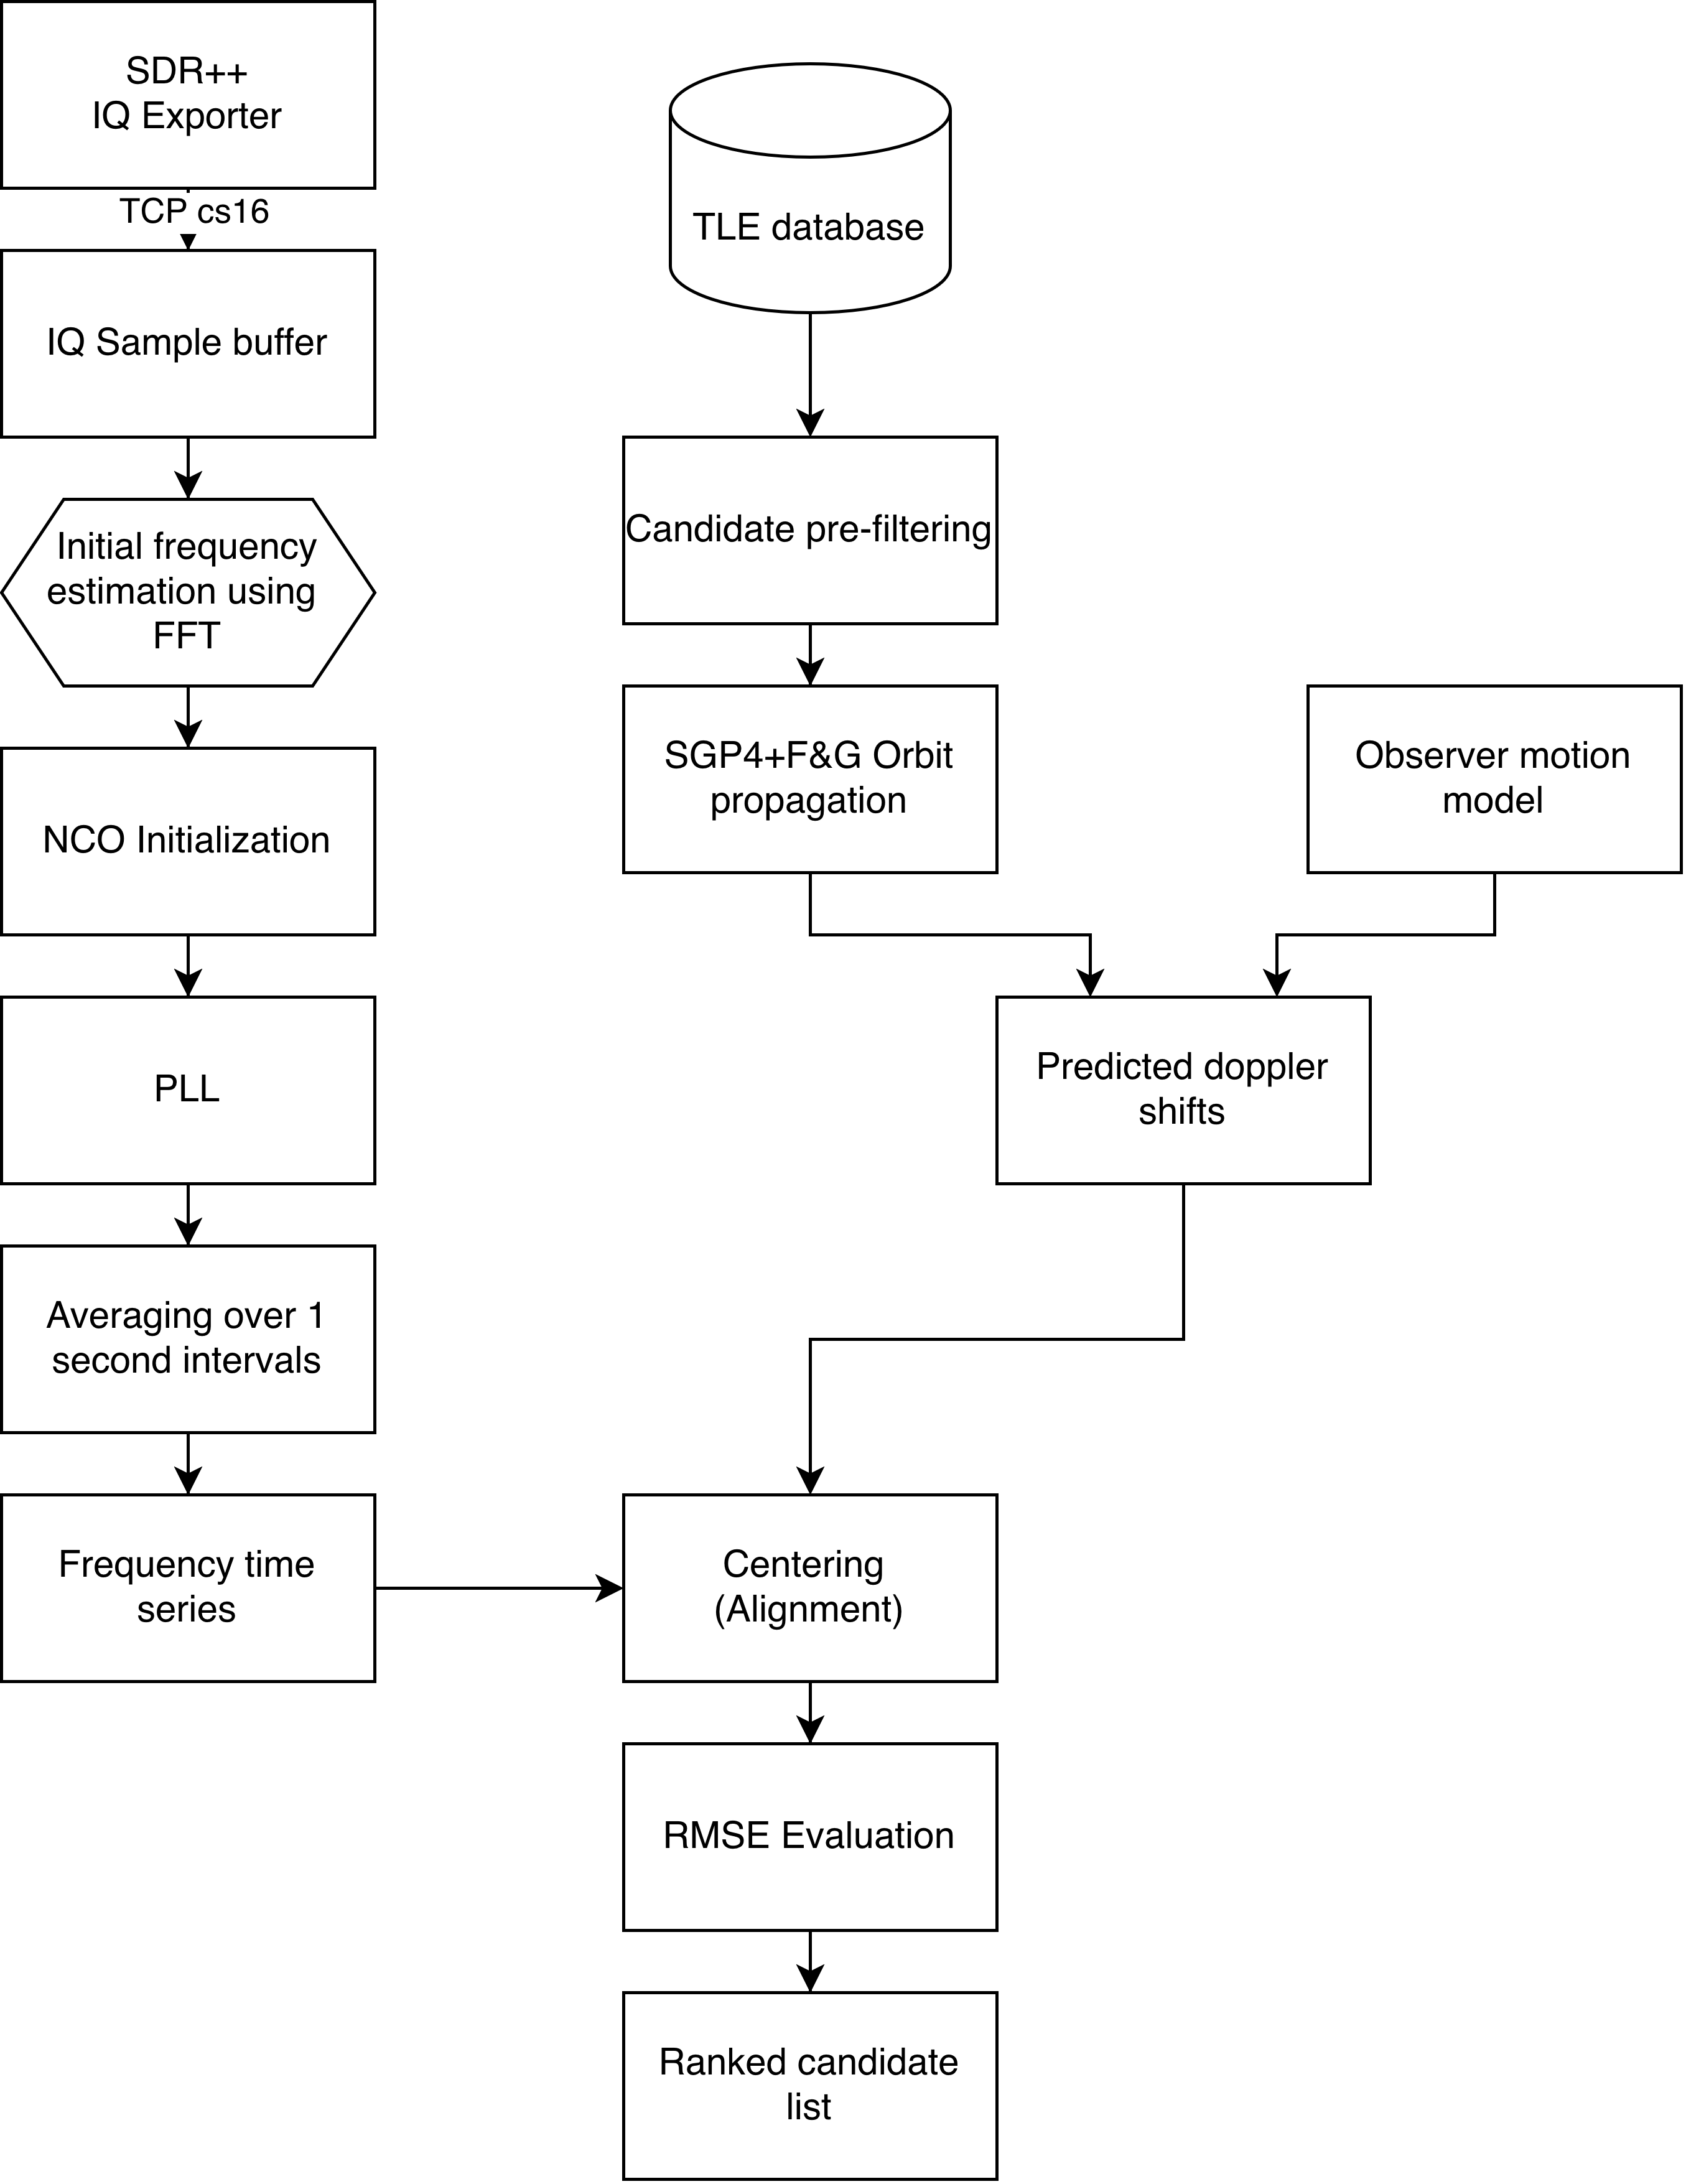
\includegraphics[width=0.95\textwidth]{fig_pipeline}
    \caption{Generalized processing chain of the passive Doppler satellite identification system.}
    \label{fig:pipeline}
\end{figure}


\subsection{Hardware and Measurement Setup}
\label{subsec:hardware}

\subsubsection{SDR Receiver Chain}
\label{subsubsec:sdr-receiver}

Three software-defined radio receivers were used in the experimental study. The first is the LibreSDR B210 mini, based on the AD9361 transceiver, with a specified reference oscillator stability of 0.5 ppm. Its architecture is close to that of the USRP B200 mini, whose characteristics are studied in detail in the study by \citet{bednarz2024}. The second is the HackRF One (Clifford R10+ revision) fitted with an external temperature-compensated crystal oscillator (TCXO) specified at 0.1 ppm. The third is the RTL-SDR v3 with a specified oscillator stability of 1 ppm. The HackRF and the B210 mini were used interchangeably for VHF, UHF, L- and S-band observations, whereas the RTL-SDR v3 was used in the L band only. No quantitative comparison between receivers was performed within the scope of this work. A GPS-disciplined oscillator (GPSDO) was intentionally excluded from the setup, as one of the objectives of this work is to demonstrate the applicability of the method on widely available consumer hardware.

The antenna front-ends varied by frequency band. In the VHF band a telescopic V-dipole antenna was used; in the UHF band a consumer-grade 7-element Yagi-Uda antenna with a folded dipole was used. Neither configuration included an external low-noise amplifier (LNA).

For the L and S bands an identical reflector, a 0.9m offset parabolic dish (AX-OFFSET D90), was used with different feeds and amplifier chains. In the L band, a left-hand circularly polarised (LHCP) helical feed, designed using an online calculator~\citep{helix_calc}, was mounted at the focal point of the reflector. Due to polarisation reversal upon reflection from a parabolic surface~\citep{kraus2002}, the system provides effective reception of right-hand circularly polarised (RHCP) signals from the source side. The receiving chain comprised a two-stage LNA with a SAW filter optimised for 1690 MHz, followed by a broadband LNA based on the TQP3M9037 transistor. In the S-band, a separate LHCP helical feed designed by the same method was used together with the SeLNA v1 LNA~\citep{selna_v1}, a modified ADS-B LNA with replacement bandpass filters adapted for 2200-2300 MHz. The two receiving chains are shown in Figure~\ref{fig:rf_chains}.

\begin{figure}[!htbp]
    \centering
    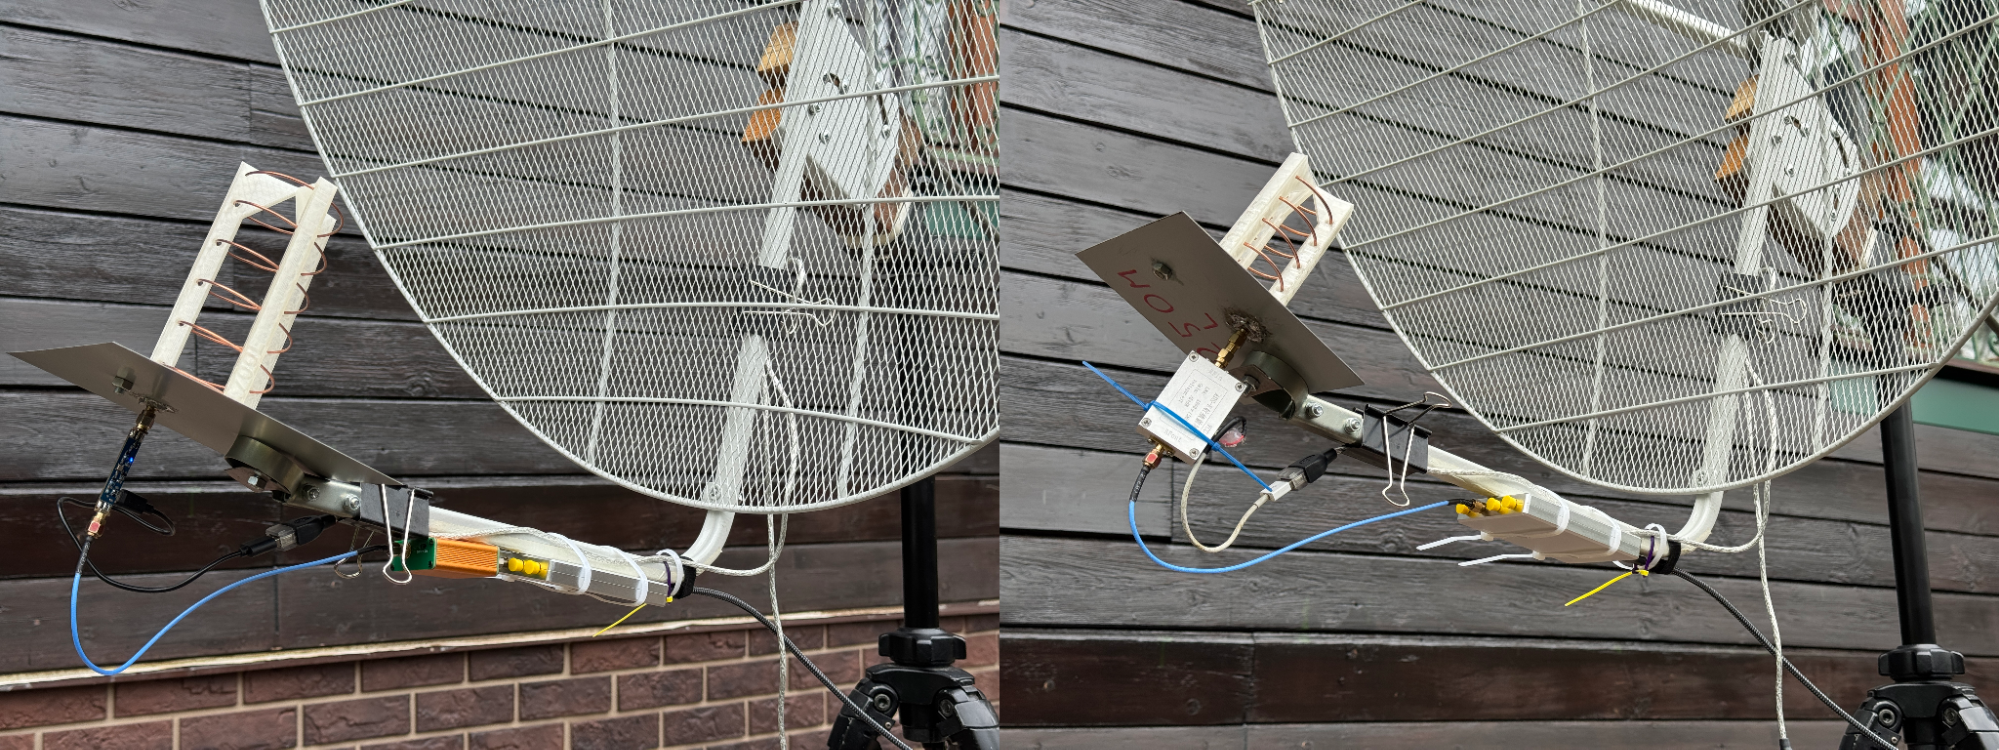
\includegraphics[width=0.95\textwidth]{fig_rf_chains_l_s}
    \caption{Photograph of the L-band (left) and S-band (right) receiving chains.}
    \label{fig:rf_chains}
\end{figure}


\subsubsection{Reference Frequency Stability Assessment}
\label{subsubsec:freq-stability}

A key source of systematic error in Doppler measurements is the instability of the SDR receiver's reference oscillator. As reported by \citet{bednarz2024}, even receivers with specified stability of 0.5--1 ppm exhibit both constant frequency offsets and slow thermal drift. The present experiments confirmed that the frequency readings of both receivers are sensitive to ambient temperature: the best results were obtained under stable thermal conditions, whereas noticeable drift was observed during transient phases such as equipment warm-up.

The presence of a constant frequency offset in both receivers was qualitatively confirmed by briefly observing the downlink signal of the geostationary satellite SBIRS-GEO 1 (SATCAT No. 37481) at 2262.5 MHz. Because the Doppler shift of a geostationary satellite is negligible compared to SDR oscillator instability, any observed frequency offset can be attributed to the systematic error of the receiver reference. This measurement was indicative only and does not constitute a quantitative characterization of oscillator stability.

None of these error sources is eliminated by hardware calibration in the present work. Instead, constant offset is compensated algorithmically through the series-centering operation applied to both the observed and predicted series, as described in Section~\ref{subsubsec:normalisation}. This approach removes the dependence of the method on an ultrastable reference oscillator and preserves its operability across a broad class of consumer SDR platforms.


\subsection{Doppler Signature Extraction}
\label{subsec:doppler-extraction}

\subsubsection{IQ Data Stream and Preprocessing}
\label{subsubsec:iq-preprocessing}

Complex IQ samples are sent to the application from the SDR++ IQ-Exporter module over TCP, with the application acting as client. Samples are transmitted in the \texttt{cs16} format (pairs of signed 16-bit integers encoding the I and Q quadrature components). The sample rate and center frequency are queried dynamically from the SDR++ \texttt{rigctl} server module via the rigctl protocol, eliminating the need for manual configuration. Incoming samples are accumulated in a fixed-size internal ring buffer before being passed to subsequent processing stages. No additional filtering or decimation is applied at this stage. The full sample stream is forwarded as-is to the frequency estimation block.


\subsubsection{Initial Frequency Estimation via FFT}
\label{subsubsec:fft-estimation}

Before the phase-locked loop is started, an optional initial frequency estimate is computed via the Discrete Fourier Transform. This step is intended for signals containing a distinct carrier and can substantially accelerate PLL lock~\citep{gao2016}. When enabled, the application accumulates samples for one second and computes the amplitude spectrum via FFT. The spectral bin with the maximum amplitude is taken as the initial carrier frequency estimate $f_0$, which is used to initialise the NCO:

\begin{equation}
    f_0 = \arg\max_k |X[k]|
    \label{eq:fft-init}
\end{equation}

\noindent
where $X[k]$ is the complex spectrum of the input sample block. In the event that this step is skipped, for signals without a distinct carrier where peak finding is not meaningful for example, the NCO is initialised with zero offset relative to the receiver center frequency.

\subsubsection{Signal Tracking via Phase-Locked Loop (PLL)}
\label{subsubsec:pll-tracking}

The primary tool for extracting the instantaneous signal frequency is a phase-locked loop implemented as a C++ module with a Python interface via pybind11. Unlike classical demodulation schemes, this implementation uses the PLL in frequency estimation mode. Here the output is the current estimate of the instantaneous signal frequency rather than a recovered phase or demodulated data~\citep{guo2015, gao2016}.

Before the loop is initialised, the maximum permissible frequency deviation from the center frequency $f_{\max}$ is computed. This is the range within which the PLL can acquire and track the signal:

\begin{equation}
    f_{\max} = \left(\frac{c + v_0}{c - v_s} - 1\right) \cdot f_{\mathrm{sat}} \cdot M
    \label{eq:fmax}
\end{equation}

\noindent
For the worst case (maximum Doppler shift), a satellite at 100 km altitude with $v_s \approx 7850$~m/s and an observer moving toward it at the Earth's equatorial rotation speed $v_0 \approx 465$~m/s,this simplifies to:

\begin{equation}
    f_{\max} \approx 2.8 \times 10^{-5} \cdot f_{\mathrm{sat}} \cdot M
    \label{eq:fmax-approx}
\end{equation}

\noindent
where $M > 1$ is a user-defined capture-range expansion factor that compensates for frequency tuning inaccuracy and reference oscillator instability in both the receiver and transmitter.

The key parameter of a PLL is the loop bandwidth, which determines the trade-off between signal acquisition speed and noise suppression. A wide bandwidth enables fast lock but requires a higher signal-to-noise ratio, whereas a narrow bandwidth provides accurate tracking of a weak signal but slows initial acquisition~\citep{guo2015}. The implementation provides a set of pre-configured bandwidth values that the operator can switch during an observation. The typical strategy in the L and S bands is to use a 2,000Hz bandwidth for initial lock, then narrow to 300Hz for fine tracking. In the VHF and UHF bands, proportionally smaller values were used, which empirically provided stable tracking.

The PLL output is subject to noise from phase jitter and dynamic tracking error, the dominant source of which is thermal noise in the receiving chain~\citep{kaplan2006}.

\subsubsection{Formation of the Frequency Time Series}
\label{subsubsec:freq-timeseries}

To suppress noise in the PLL output stream, a one second averaging procedure is applied. All frequency samples $f_i$ arriving in the interval $[N - 0.5,\; N + 0.5)$, where $N$ is an integer Unix timestamp, are averaged into a single value:

\begin{equation}
    \hat{f}(N) = \frac{1}{|S_N|} \sum_{i \in S_N} f_i,
    \qquad S_N = \{i : |t_i - N| < 0.5\}
    \label{eq:averaging}
\end{equation}

The result is a time series $\{(N_j,\, \hat{f}(N_j))\}$ representing the Doppler signature of the observed signal sampled at one second intervals. This gets fed into the identification algorithm described in Section~\ref{subsec:identification-algorithm}.

\subsection{Generation of Predicted Doppler Trajectories}
\label{subsec:predicted-trajectories}

\subsubsection{TLE Acquisition and Processing}
\label{subsubsec:tle-processing}

Two-Line Element sets are obtained from several configurable sources. The first is CelesTrak, which provides the active satellite catalog through an open API. The second is ReTLEctor~\citep{retlector}, a lightweight proxy server that caches CelesTrak data to prevent rate-limit violations during bulk downloads. The third is Space-Track, the official catalog of the US Space Forces Command, from which records with an epoch no older than 14 days and no decay date are requested. The fourth is the Mike McCants archive~\citep{mmccants}, which contains unofficial TLE data for satellites absent from official catalogs but identified through legitimate passive observations (this source does not redistribute classified data). Finally, a user-supplied plain text file of TLE sets allows arbitrary orbital elements to be included optionally.

The retrieved data is stored in a local database. When the same satellite appears in multiple sources, the entry with the most recent epoch is kept. The database is updated manually by the operator before each observing session. Local caching removes the dependency on external API availability at identification time and avoids latency from real-time network requests.


\subsubsection{Orbit Propagation via SGP4 + F\&G Functions}
\label{subsubsec:sgp4-fg}

Predicted Doppler trajectory generation is performed in two stages to minimise computational cost.

In the first stage, for each candidate object that has passed the initial filtering, the SGP4 model~\citep{vallado2006} is called once to compute the position and velocity vector at the initial observation epoch $t_0$:

\begin{equation}
    \mathbf{r}_{\mathrm{sat}}(t_0),\;\mathbf{v}_{\mathrm{sat}}(t_0)
    = \mathrm{SGP4}(\mathrm{TLE},\,t_0)
    \label{eq:sgp4-call}
\end{equation}

If the Doppler pre-filter is enabled (Section~\ref{subsubsec:prefiltering}), the computed state is used to calculate one predicted Doppler offset at $t_0$ and immediately reject candidates that do not pass, without propagating the full orbit. The result is also used for the visibility filter. These two steps are the last in the filtering chain.

In the second stage, for objects that pass all filters, the orbit is propagated over the full observation interval using F\&G functions~\citep{sharifi2011, seif2017}. At each epoch $t_0 + \Delta t$ the new state vector is computed independently from the initial state $(\mathbf{r}_0, \mathbf{v}_0)$:

\begin{equation}
    \mathbf{r}(t_0 + \Delta t) = f\,\mathbf{r}_0 + g\,\mathbf{v}_0
    \label{eq:fg-r}
\end{equation}
\begin{equation}
    \mathbf{v}(t_0 + \Delta t) = \dot{f}\,\mathbf{r}_0 + \dot{g}\,\mathbf{v}_0
    \label{eq:fg-v}
\end{equation}

The coefficients $f$, $g$, $\dot{f}$, $\dot{g}$ are computed from the change in eccentric anomaly $\Delta E$, which is found from the generalized Kepler equation by Newton-Raphson iteration:

\begin{equation}
    n\,\Delta t = \Delta E
        - \left(1 - \frac{r_0}{a}\right)\sin(\Delta E)
        + \frac{\mathbf{r}_0 \cdot \mathbf{v}_0}{\sqrt{\mu a}}
          \left(1 - \cos(\Delta E)\right)
    \label{eq:kepler}
\end{equation}

\noindent
where $a$ is the semi-major axis, $n = \sqrt{\mu/a^3}$ is the mean motion, and $\mu = 3.986004418 \times 10^{5}$ km$^3$/s$^2$ is the Earth's standard gravitational parameter. Iteration terminates when the convergence criterion $|\delta(\Delta E)| < 10^{-12}$ rad is satisfied, or after a maximum of 10 iterations. Once $\Delta E$ is found, the coefficients are evaluated as:

\begin{equation}
    f = 1 - \frac{a}{r_0}(1 - \cos\Delta E),
    \qquad
    g = \Delta t - \sqrt{\frac{a^3}{\mu}}(\Delta E - \sin\Delta E)
    \label{eq:fg-coeff-fg}
\end{equation}
\begin{equation}
    \dot{f} = -\frac{\sqrt{\mu a}}{r\,r_0}\sin\Delta E,
    \qquad
    \dot{g} = 1 - \frac{a}{r}(1 - \cos\Delta E)
    \label{eq:fg-coeff-dotfg}
\end{equation}

To reduce computational cost, satellite and observer positions are precomputed and cached for 1,000 consecutive seconds starting from $t_0$, which covers the typical duration of observable LEO passes. When the Doppler shift at a specific epoch is requested, the corresponding state vectors are retrieved from the cache without recomputation.


\subsubsection{Observer Motion Model}
\label{subsubsec:observer-model}

The precise observer position in the GCRS frame at the initial epoch $t_0$ is computed using the Skyfield library, accounting for Earth's precession and nutation. For all subsequent epochs $t = t_0 + \Delta t$, the observer coordinates are obtained by rotating the ITRS vector by the angle corresponding to elapsed time:

\begin{equation}
    \mathbf{r}_{\mathrm{obs}}(t)
    = \mathbf{R}_z(\omega_\oplus\,\Delta t)\,
      \mathbf{R}_{\mathrm{ITRS}\to\mathrm{GCRS}}(t_0)\,
      \mathbf{r}_{\mathrm{ITRS}}
    \label{eq:observer-pos}
\end{equation}

\noindent
where $\omega_\oplus = 7.2921150 \times 10^{-5}$ rad/s is the Earth's rotation rate. The observer velocity in the GCRS frame is:

\begin{equation}
    \mathbf{v}_{\mathrm{obs}}
    = \boldsymbol{\omega}_\oplus \times \mathbf{r}_{\mathrm{obs}}
    = \begin{bmatrix} -\omega_\oplus\,y \\ \omega_\oplus\,x \\ 0 \end{bmatrix}
    \label{eq:observer-vel}
\end{equation}

This approximation neglects small variations in Earth's rotation axis orientation over the observation interval, which is well justified for typical LEO pass durations of 10-15 minutes.


\subsubsection{Computation of the Predicted Doppler Shift}
\label{subsubsec:predicted-doppler}

At each observation epoch the predicted Doppler shift is computed from the projection of the relative velocity vector onto the line of sight. The unit line of sight vector is:

\begin{equation}
    \hat{\boldsymbol{\rho}}
    = \frac{\mathbf{r}_{\mathrm{sat}} - \mathbf{r}_{\mathrm{obs}}}
           {|\mathbf{r}_{\mathrm{sat}} - \mathbf{r}_{\mathrm{obs}}|}
    \label{eq:los-unit}
\end{equation}

The radial approach velocity along the line of sight is:

\begin{equation}
    \dot{\rho}
    = (\mathbf{v}_{\mathrm{obs}} - \mathbf{v}_{\mathrm{sat}})
      \cdot \hat{\boldsymbol{\rho}}
    \label{eq:rdot}
\end{equation}

\noindent
where a positive $\dot{\rho}$ corresponds to mutual approach. Using the first-order approximation from Section~\ref{subsec:doppler-shift}, the predicted observed frequency is:

\begin{equation}
    f_{\mathrm{pred}} = f_{\mathrm{sat}}
        \left(1 + \frac{\dot{\rho}}{c}\right)
    \label{eq:fpred}
\end{equation}

Since the exact transmitter carrier frequency $f_{\mathrm{sat}}$ is generally unknown, the absolute values of $f_{\mathrm{pred}}$ are not used directly in the matching algorithm. Instead, both the observed and predicted series are centered by subtracting their respective means, as described in Section~\ref{subsubsec:normalisation}.


\subsection{Satellite Identification Algorithm}
\label{subsec:identification-algorithm}

\subsubsection{Prefiltering of Candidate Satellites}
\label{subsubsec:prefiltering}

The TLE catalog currently contains approximately 15,000 objects, for which full orbit propagation is impractical. To reduce the candidate set to a manageable size, sequential multi-stage filtering is applied. The seven filters are ordered by increasing computational cost.

The first five filters operate directly on TLE fields without invoking the propagation model. The \emph{debris filter} rejects objects whose name contains the substrings \texttt{deb}, \texttt{rb}, or \texttt{r/b} (case insensitive), eliminating known debris and rocket bodies. The \emph{epoch filter} rejects ephemerides older than a configurable threshold (14 days by default), as propagating such old elements with the SGP4 model yields unacceptable prediction accuracy. The \emph{constellation filter} excludes satellites belonging to mega-constellations (by default Starlink and OneWeb), as their signals are largely inaccessible to passive reception in the bands under study. The \emph{GEO and high-orbit filter} rejects objects with mean motion $n < 6$ revoulutions per day, a threshold chosen empirically because the expected Doppler shift for such orbits is substantially lower than for LEO objects and carries little to no discriminating information over short observation intervals. The \emph{high eccentricity filter} excludes objects with eccentricity $e > 0.25$, a threshold chosen empirically as a compromise between reducing the candidate count and retaining observable objects.

For the remaining objects, SGP4 is called once to compute the position and velocity vector at the initial observation epoch $t_0$. The result is shared by the two subsequent filters. The \emph{visibility filter} rejects satellites with elevation below the horizon $\theta_{\mathrm{el}} < \theta_{\min}$ (default: $0^\circ$) at $t_0$, restricting the candidate set to objects that were above the horizon at the start of the observation. Finally, the \emph{Doppler pre-filter} rejects satellites whose predicted Doppler shift at $t_0$ differs from the observed value by more than a configurable threshold $\varepsilon$:

\begin{equation}
    \left|\Delta f_{\mathrm{pred}}(t_0) - \Delta f_{\mathrm{obs}}(t_0)\right|
    > \varepsilon
    \label{eq:doppler-prefilter}
\end{equation}

This particular filter is most effective when the center frequency of the signal is not known precisely. In that case, its use is not recommended, as it risks incorrectly rejecting the true candidate.

\subsubsection{Trajectory Normalisation}
\label{subsubsec:normalisation}

Direct comparison of the observed and predicted frequency series is not possible for several reasons. First, the exact transmitter carrier frequency $f_{\mathrm{sat}}$ is generally unknown, introducing a constant offset between the series. Second, reference oscillator instability in the SDR receiver adds a further systematic offset and slow drift. The constant offset is removed by centering: the mean of each series is subtracted from it:

\begin{equation}
    \tilde{f}_{\mathrm{obs},i} = f_{\mathrm{obs},i} - \bar{f}_{\mathrm{obs}}
    \label{eq:center-obs}
\end{equation}
\begin{equation}
    \tilde{f}_{\mathrm{pred},i} = f_{\mathrm{pred},i} - \bar{f}_{\mathrm{pred}}
    \label{eq:center-pred}
\end{equation}

The centered series $\tilde{f}_{\mathrm{obs}}$ and $\tilde{f}_{\mathrm{pred}}$ retain only information about the shape of the Doppler curve, which is invariant to constant offsets of any origin. The operation also makes the method robust to imprecise receiver tuning. Formally, assuming:

\begin{equation}
    f_{\mathrm{obs}}(t) = f_D(t) + b + \epsilon(t)
    \label{eq:noise-model}
\end{equation}

\noindent
where $f_D(t)$ is the Doppler component, $b$ is the constant bias (unknown transmitter frequency combined with the SDR local oscillator offset), and $\epsilon(t)$ is noise, subtracting the mean gives:

\begin{equation}
    \tilde{f}_{\mathrm{obs}}(t) = f_D(t) - \bar{f}_D + \epsilon(t) - \bar{\epsilon}
    \label{eq:after-centering}
\end{equation}

\noindent
because the constant term cancels exactly: $b - \bar{b} = 0$.


\subsubsection{Matching Metric}
\label{subsubsec:matching-metric}

The proximity between the observed and predicted Doppler signatures is measured by the root mean square error (RMSE) of the centered series:

\begin{equation}
    \mathrm{RMSE} = \sqrt{\frac{1}{N}\sum_{i=1}^{N}
        \left(\tilde{f}_{\mathrm{obs},i}
            - \tilde{f}_{\mathrm{pred},i}\right)^2}
    \label{eq:rmse}
\end{equation}

\noindent
where $N$ is the number of timestamps common to both series. RMSE was chosen because the Doppler trajectories are time-synchronised and sampled simultaneously, making amplitude domain deviation the primary discriminating feature. Candidates are ranked in ascending order of RMSE, with the lowest value corresponding to the best match. Across the observations collected in this study, the RMSE of the correct object was typically several times lower than that of the second-ranked candidate, with the gap widening as observation duration increased.


\subsubsection{Computational Complexity of the Algorithm}
\label{subsubsec:complexity}

To quantify pipeline performance, 10 random observer locations and 10 random epochs were combined into 100 test cases, each of which was processed by the full pipeline with synthetic data. Mean execution times for the principal stages are shown in Figure~\ref{fig:timing}.

\begin{figure}[!htbp]
    \centering
    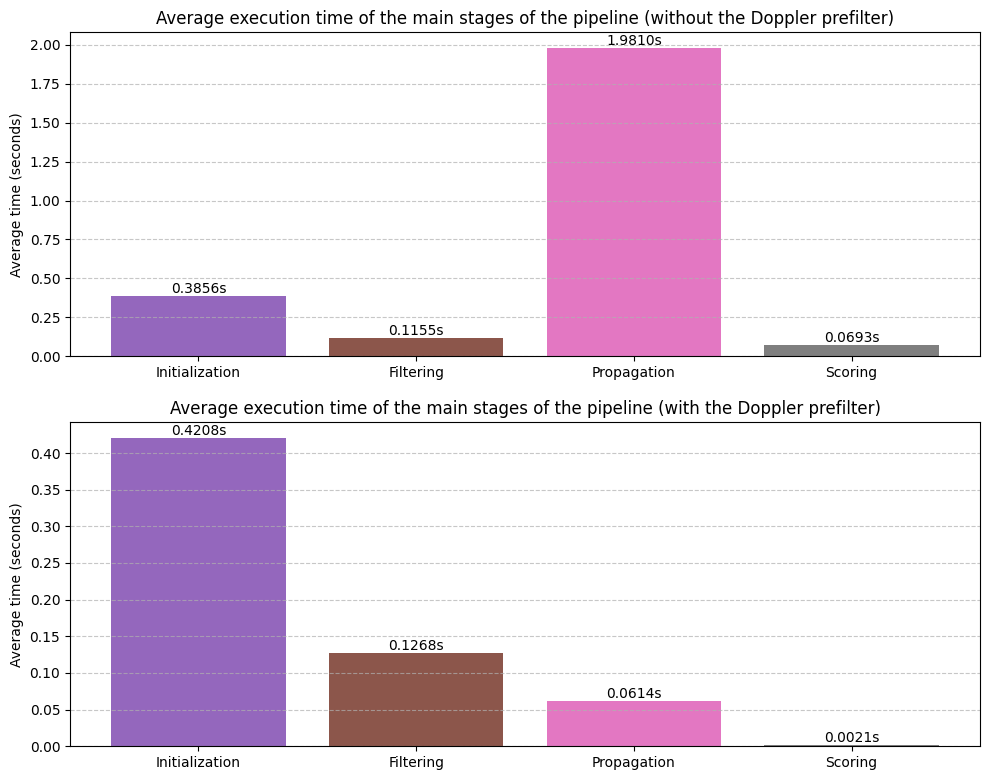
\includegraphics[width=0.95\textwidth]{fig_timing_prefilter_comparison}
    \caption{Execution time breakdown by pipeline stage, with and without the
             Doppler pre-filter.}
    \label{fig:timing}
\end{figure}

Without the pre-filter, orbit propagation is the dominant stage (78.7\% of total time), driven by Newton-Raphson iteration of the Kepler equation for each of $\sim$177 candidate satellites across 1,000 time points. Enabling the Doppler pre-filter reduces the mean number of candidates reaching the F\&G propagation stage from 176.6 to 4.7, yielding a 32-fold speedup of the propagation stage and a 4.5-fold speedup of the overall pipeline. The number of remaining candidates after each filtering step is shown in Figure~\ref{fig:filter_funnel}.

\begin{figure}[!htbp]
    \centering
    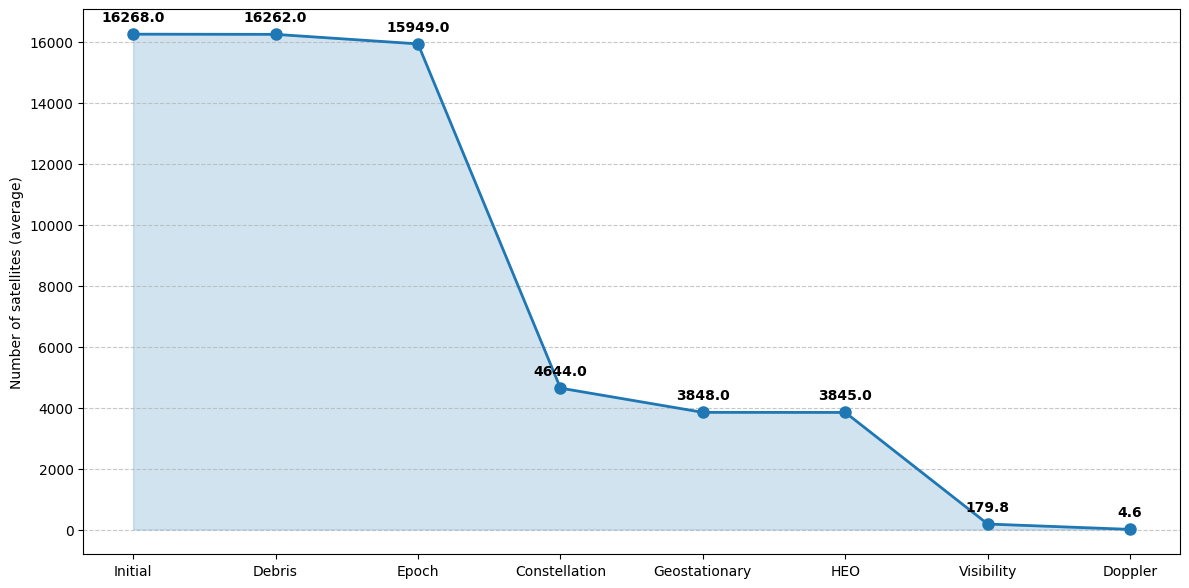
\includegraphics[width=0.95\textwidth]{fig_filter_funnel}
    \caption{Candidate count at each stage of the filtering pipeline.}
    \label{fig:filter_funnel}
\end{figure}
% ================================================================
\section{Experimental Study}
\label{sec:experiment}

\subsection{Experimental Methodology}
\label{subsec:methodology}

Observations were conducted near the town of Aprelevka, Naro-Fominsk District, Moscow Region (approximately 55.5°\,N, 37.1°\,E), over several weeks in 2026, with a total active observation time of approximately 20 hours. Both receivers described in Section~\ref{subsubsec:sdr-receiver} were used depending on equipment availability at the time of observation. Results did not differ appreciably between receivers.

Observations were conducted primarily in the evening, most often around sunset, because of the high density of passes by sun-synchronous satellites during that period. Candidate signals were identified on an opportunistic basis: the operator monitored a live spectrogram in SDR++ looking for unfamiliar signals and checked each one for a pronounced Doppler shift. It appeared as the characteristic leftward drift of spectral lines over time on the FFT plot. Signals showing no visible Doppler shift were disregarded as geostationary or terrestrial.

Before each observing session the operator manually updated the local TLE database from CelesTrak, ReTLEctor, and the Mike McCants archive. The last source was added after several early observations yielded no identification because the satellites in question were absent from the official catalogs.

Once a candidate signal was detected, the tripod-mounted antenna was pointed at the source manually. In the UHF, L, and S bands, tracking throughout the pass was maintained by continuously adjusting the antenna direction against the signal level on the FFT display, with a drop in amplitude indicating pointing error. In the VHF band a fixed V-dipole antenna was used without mechanical tracking. The center frequency of the IQ Exporter in SDR++ was set approximately to the observed signal with a downward correction for Doppler shift: since the signal frequency decreases on the descending portion of the pass, the tuning was placed slightly below the observed carrier. The FFT-based initial frequency estimation was enabled where needed. The PLL capture bandwidth was set to 1,000-2,000 Hz for initial lock, then narrowed to 300 Hz for fine tracking in the L and S bands; proportionally smaller values were used at lower frequencies.

A typical pass lasted approximately 5 minutes, though recorded passes ranged from 50 seconds to 10 minutes depending on maximum elevation and observing conditions. The identification algorithm described in Section~\ref{subsec:identification-algorithm} was run live during each pass.

Identification correctness was verified in two stages. First, the antenna pointing direction at the time of observation was compared against the predicted azimuth and elevation of the identified satellite in GPredict, where agreement confirmed the plausibility of the result. Second, the next pass of the identified satellite was predicted from its TLE and observed independently. Successful tracking with a consistent Doppler curve served as the final confirmation. All 28 repeat observations were successful. Cases in which the algorithm did not produce a confident identification are discussed below.


\subsection{Satellite Identification Results}
\label{subsec:results}

The experimental dataset comprises 28 successful identifications of LEO satellites across the VHF, UHF, L, and S bands: 2 observations in VHF, 1 in UHF, 3 in L, and 22 in S. In every case identification was performed from a single pass, without external receiver frequency calibration and without activating the Doppler pre-filter. Systematic bias was removed solely through the series centering procedure described in Section~\ref{subsubsec:normalisation}.

In all observations the correct satellite ranked first by the RMSE metric. Results for a representative sample from each band are given in Table~\ref{tab:results}.

\begin{table}[!htbp]
    \centering
    \caption{Identification results for a representative sample of satellites.}
    \label{tab:results}
    \begin{tabular}{lrrrrr}
        \toprule
        Satellite & SATCAT No. & Frequency (MHz) & RMSE$_1$ (Hz) & RMSE$_2$ (Hz) \\
        \midrule % nums in google sheets
        METEOR-M2 4         & 59051 & 137.9   &  4.39 &   45.22 \\
        IONOSFERA-M 3       & 64876 & 150     &  8.25 &  174.90 \\
        IONOSFERA-M 4       & 64877 & 400     &  5.49 &  509.64 \\
        SARAL               & 39086 & 1698.4  & 50.20 &  773.46 \\
        METEOR-M2 3 (TX1)   & 57166 & 1700    & 40.70 &  460.24 \\
        METEOR-M2 3 (TX2)   & 57166 & 1544.5  & 28.59 & 1032.61 \\
        FENGYUN 3F          & 57490 & 2264.65 & 28.28 & 1928.28 \\
        HINODE (SOLAR-B)    & 29479 & 2256.22 & 24.89 & 1525.86 \\
        METOP-B             & 38771 & 2230    & 75.24 &  690.29 \\
        PROBA-2             & 36037 & 2235    &268.87 & 1039.19 \\
        \bottomrule
    \end{tabular}
\end{table}

Across all bands, the RMSE of the true object is substantially lower than that of the nearest false candidate. In the S band, where the largest number of observations was accumulated ($n = 22$), the mean ratio RMSE$_1$/RMSE$_2$ was 0.073, while the mean ratio RMSE$_2$/RMSE$_3$ was 0.732, indicating a sharply defined minimum of the error function at the correct candidate. A similar pattern holds in the L band ($n = 3$): mean RMSE$_1$/RMSE$_2 = 0.060$ against RMSE$_2$/RMSE$_3 = 0.664$. Averaging across the VHF and UHF bands is not meaningful given the small sample sizes. Individual values for those cases are listed directly in Table~\ref{tab:results}. The table shows that even when the absolute Doppler shift is small at lower frequencies, the shape of the trajectory remains sufficient for confident discrimination between spacecraft.

The largest number of observations was made in the S band, due to the sheer number of available signals and the high discriminating power of their doppler signatures. For FENGYUN 3F, for instance, the gap between RMSE$_1$ and RMSE$_2$ exceeds two orders of magnitude. Results in the L and UHF bands are comparable in quality. In the S band, four satellites of the CENTISPACE constellation were additionally identified on different frequencies, demonstrating that the method generalizes across multiple signals within a single constellation.

A notable case is the observation of METOP-B, which was successfully identified at the beginning of its pass during the initial testing and development of the application. Later in the pass, when the spacecraft's coherent transponder locked onto an uplink from the ground station, the observed downlink acquired a double Doppler shift: the uplink experiences Doppler on the ground-to-space path, and the coherently retransmitted downlink experiences Doppler again on the space-to-ground path~\citep{dsn810005_202}. This resulted in an abrupt change in the observed Doppler trajectory, causing the identification algorithm to fail. The case clearly illustrates one of the method's limitations, discussed below.

The effect of TLE age on identification accuracy is illustrated by PROBA-2, for which RMSE$_1$ was 268.87 Hz, which is substantially higher than the values typical of other observations due to the use of outdated ephemerides. Nevertheless, the correct object retained first place in the ranking with RMSE$_2 = 1039.19$ Hz, indicating robustness of the method to moderate ephemeris errors. A corresponding example output is shown in Figure~\ref{fig:proba2}.

\begin{figure}[!htbp]
    \centering
    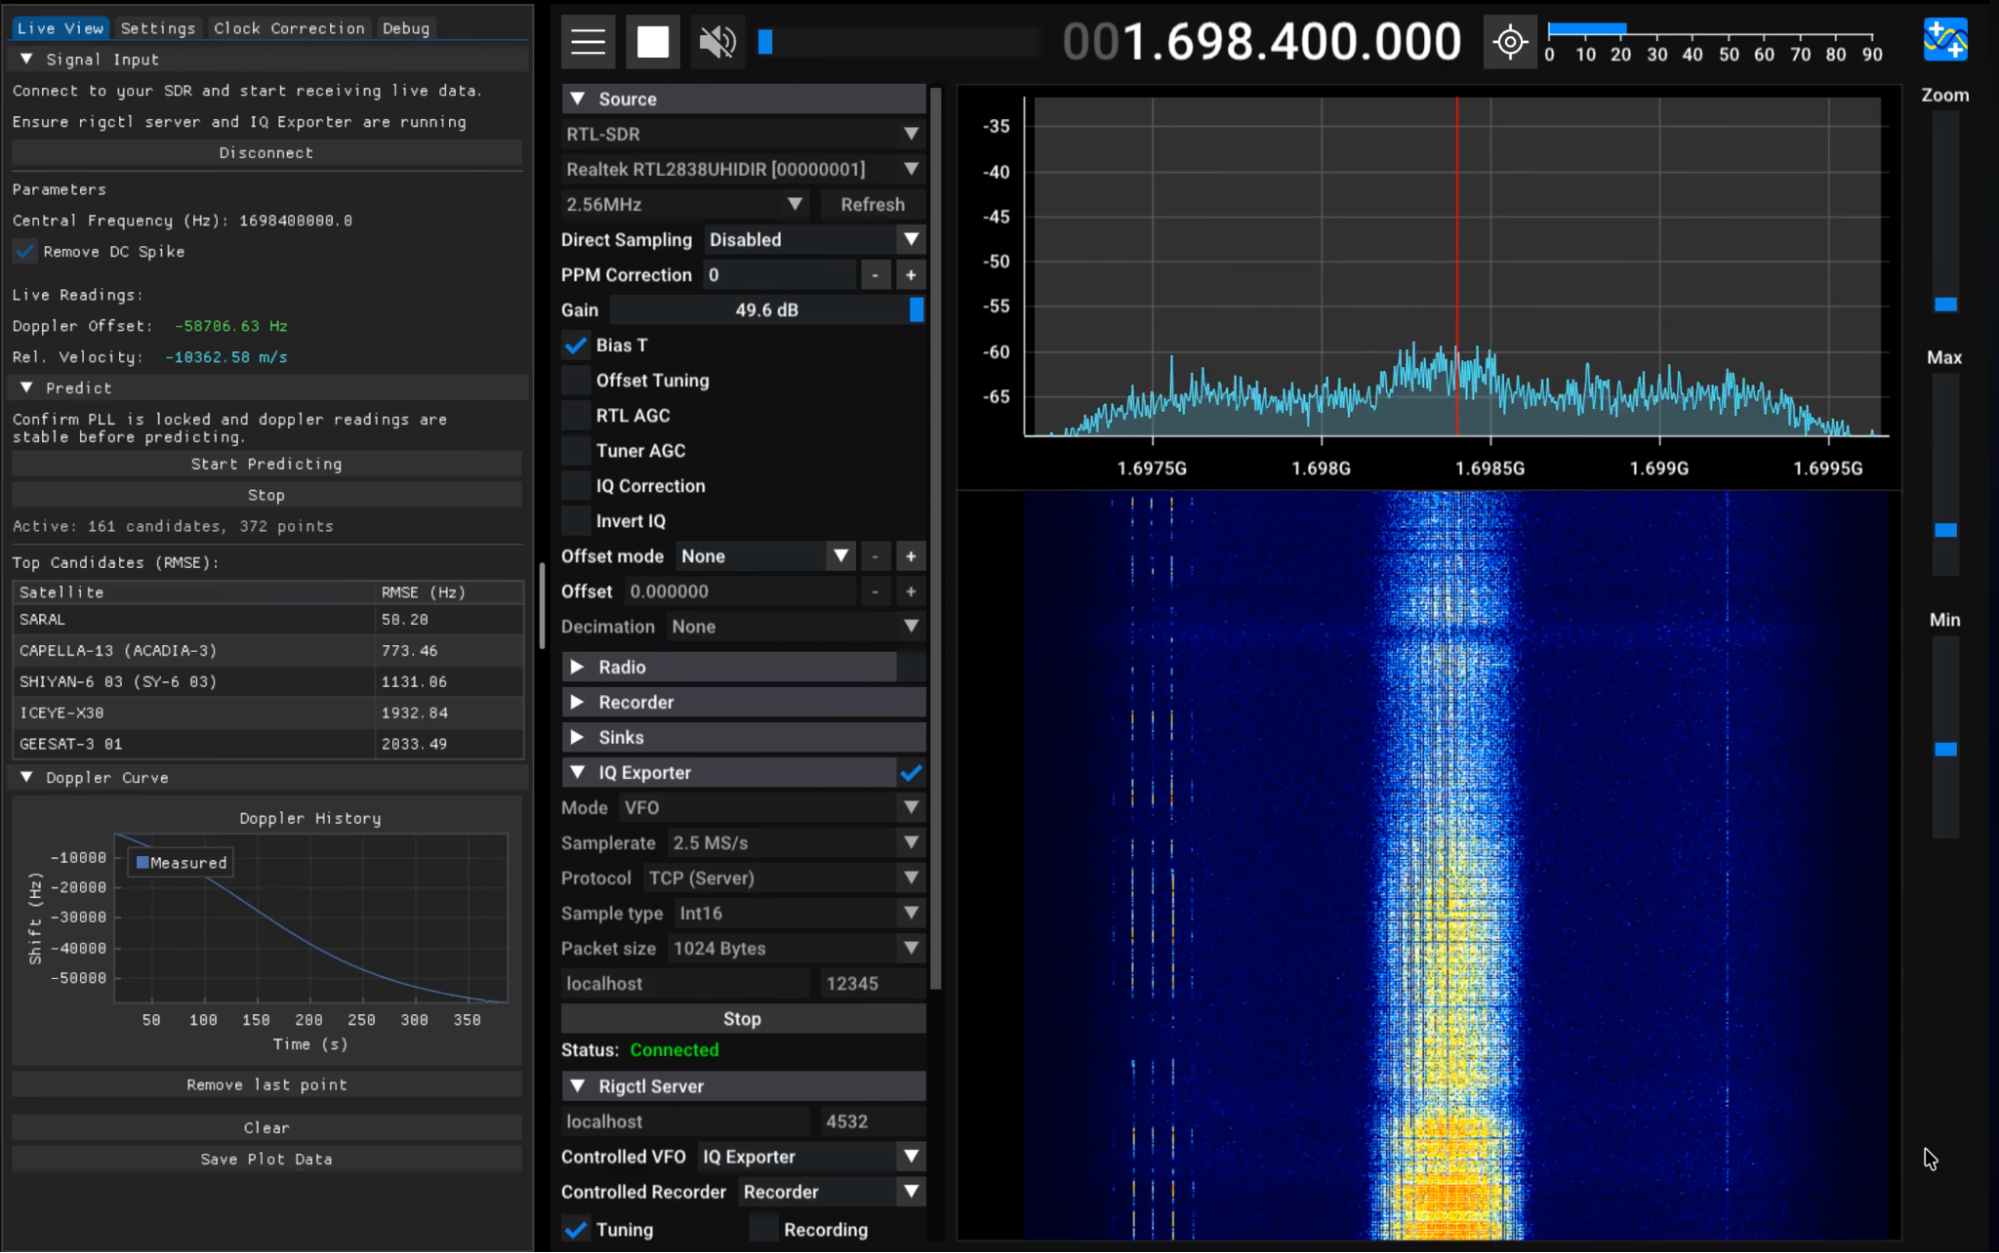
\includegraphics[width=0.95\textwidth]{fig_saral_lband}
    \caption{Identification of SARAL in the L band.}
    \label{fig:saral}
\end{figure}

\begin{figure}[!htbp]
    \centering
    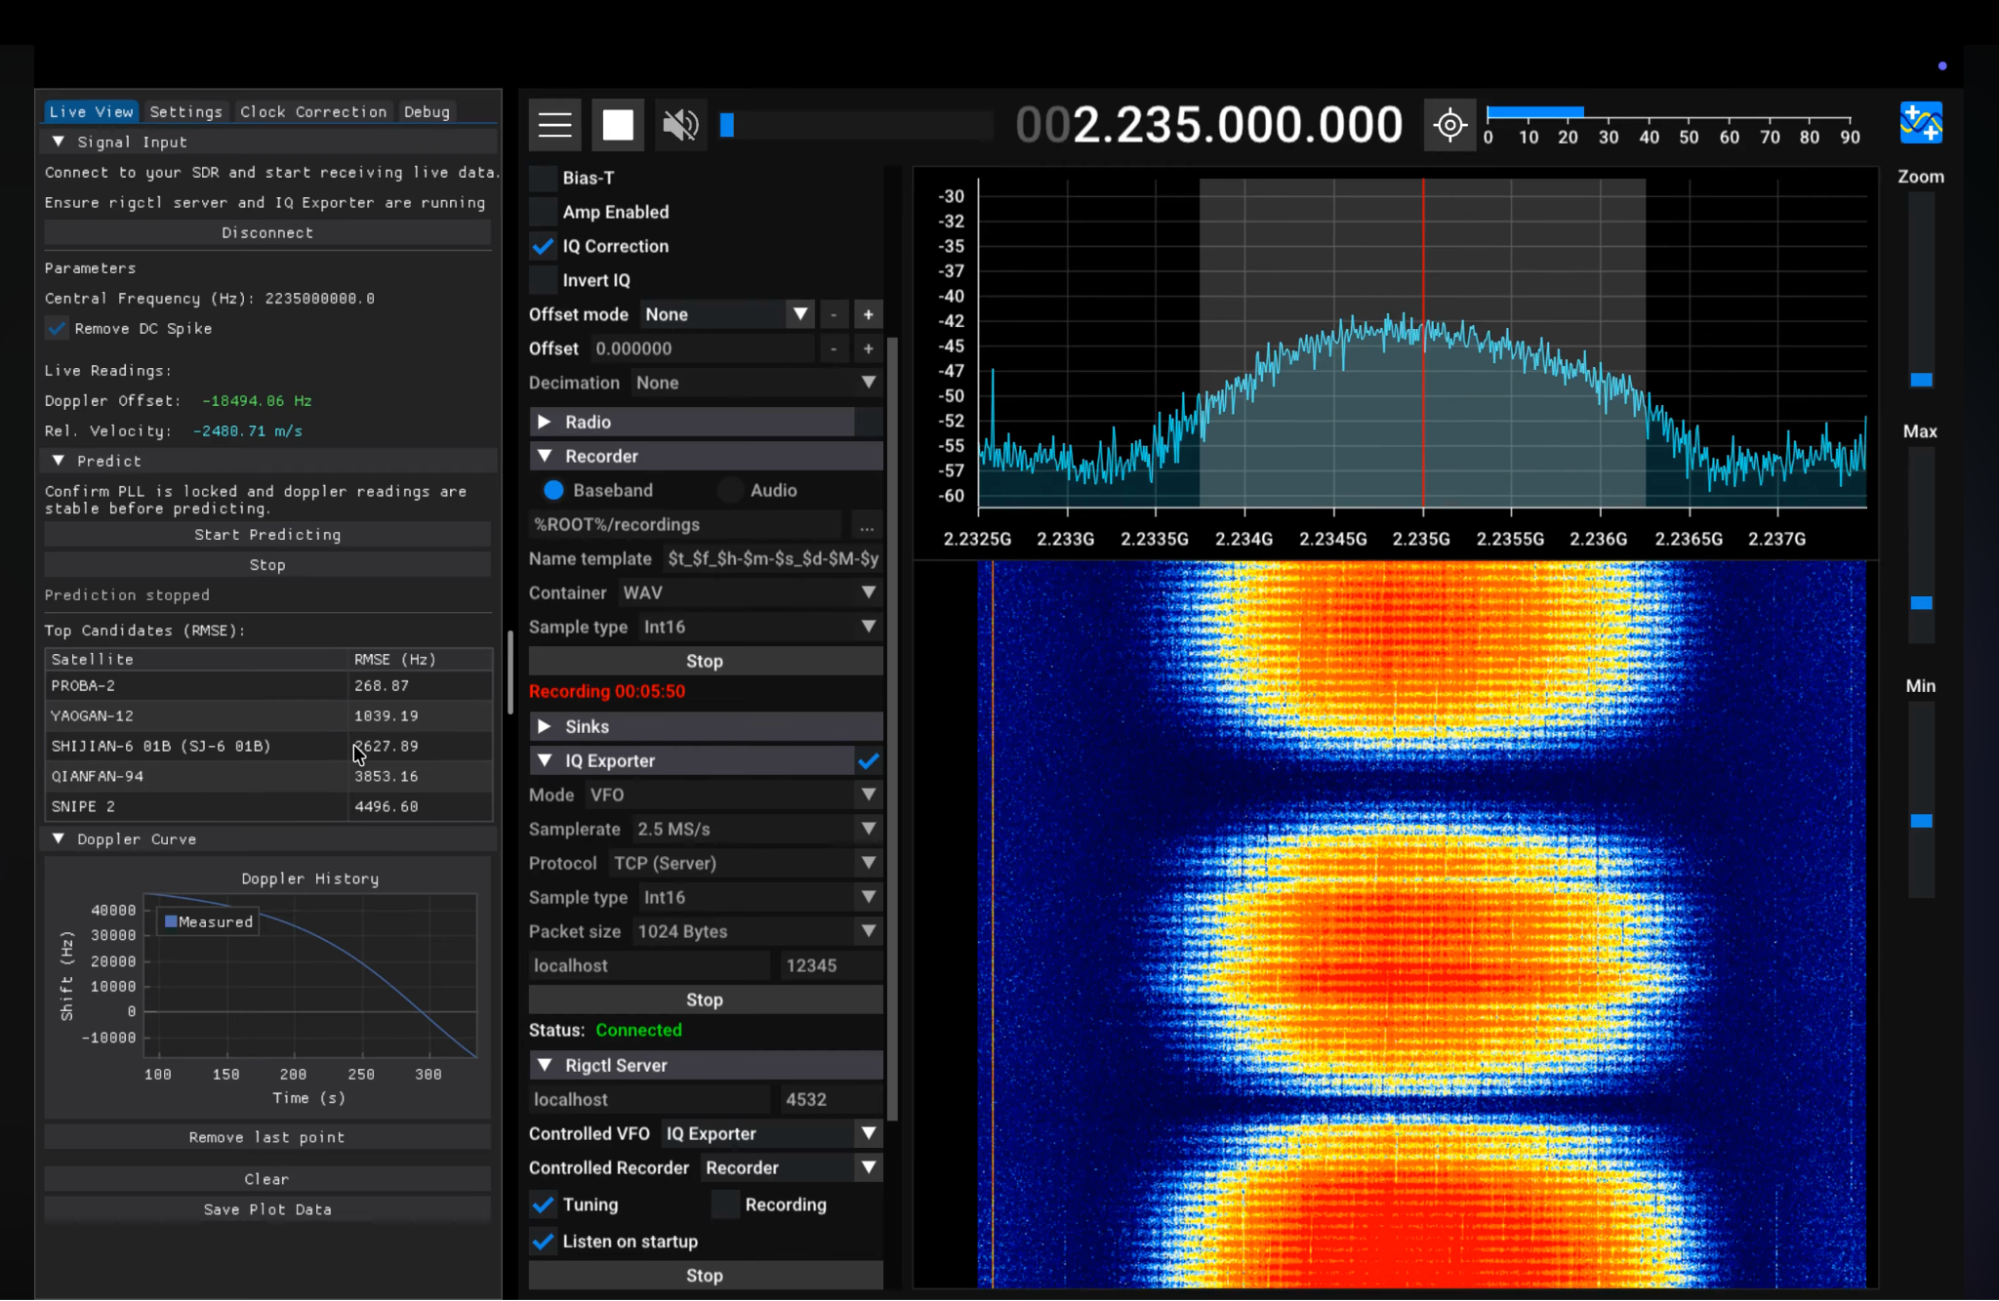
\includegraphics[width=0.95\textwidth]{fig_proba2_old_tle}
    \caption{Identification of PROBA-2 with outdated TLE data.}
    \label{fig:proba2}
\end{figure}

Three characteristic failure modes were identified during the observations. The first is coherent transponder operation, illustrated above by the METOP-B case. The second is the absence of a satellite from certain TLE catalogs: the most notable examples are the NOSS-3 satellites, which do not appear in official open sources but are present in the Mike McCants archive. In such cases correct identification is impossible without including that ephemeris source. The third failure mode is insufficient signal-to-noise ratio: under deep signal fades the PLL loses lock, which corrupts the frequency time series. Identification is also degraded for short transmissions, namely brief data-dump sessions or burst-mode transmissions, where the observed Doppler trajectory is too short for confident discrimination between candidates.

Taken together, the results confirm that passive satellite identification from a single pass is achievable with consumer grade SDR receivers across a wide frequency range, from VHF through S band, without external frequency calibration and without precise knowledge of the signal carrier frequency.

% ================================================================

\section{Discussion and Conclusion}
\label{sec:conclusion}

\subsection{Main Findings}
\label{subsec:findings}

This work presents a method for passive satellite identification from the Doppler signature of a single pass, developed and experimentally validated in full. All objectives stated in the introduction have been addressed.

A Doppler signature extraction method was developed based on a phase-locked loop implemented as a high-throughput processing module. The validity of the first-order approximation relating Doppler shift to relative velocity was established for LEO satellite observation scenarios. A computationally efficient approach to generating predicted Doppler trajectories was proposed, combining a single SGP4 call with subsequent orbit propagation via F\&G functions. A trajectory matching algorithm was developed based on the RMSE metric with mean-subtraction normalisation, which simultaneously compensates for the unknown transmitter carrier frequency, the constant offset of the receiver reference oscillator, and its slow drift. The compensation procedure was thus confirmed to work without external frequency references or GPS-disciplined oscillators.

The method was experimentally validated on 28 satellites across the VHF, UHF, L,and S bands using consumer-grade SDR receivers. In every case the correct spacecraft ranked first by RMSE with a clear margin over the nearest false candidate.

The proposed method has no direct counterpart among the approaches reviewed in the literature. Its implementation on consumer SDR hardware makes it broadly accessible for applications in radio astronomy, post-deployment identification of small satellites, and radio-frequency spectrum monitoring.


\subsection{Directions for Further Development}
\label{subsec:future-work}

The most immediate avenue for development is automation of the receiving chain through integration of the antenna with a motorised rotator driven by predicted orbital elements or signal to noise ratio of the unidentified signal in real time. This would replace manual satellite tracking with a fully autonomous observation mode and remove the dependence of signal quality on operator input.

A significant functional extension would be support for burst transmissions. The current implementation assumes a continuous signal with a stable carrier suitable for PLL tracking. Adapting the method to short burst transmissions would require an alternative frequency estimation block - for instance, frame by frame FFT followed by aggregation of the individual frequency estimates into a single Doppler curve.

A promising direction for improving identification robustness is the inclusion of antenna pointing angles as an additional observable. If the antenna direction corresponding to the signal maximum is recorded throughout a pass, the resulting angular trajectory can serve as an independent constraint during candidate matching: satellites whose predicted angular trajectory diverges from the observed one can be rejected even when their Doppler RMSE is low. Combining Doppler and angular observables could substantially reduce the probability of false identification in high orbital density environments.

% =================================================================
\bmhead{List of abbreviations}
\begin{description}
    \item [ADS-B] Automatic Dependent Surveillance-Broadcast
    \item [API] Application Programming Interface
    \item [CCSDS] Consultative Committee for Space Data Systems
    \item [FFT] Fast Fourier Transform
    \item [GCRS] Geocentric Celestial Reference System
    \item [GEO] Geostationary Earth Orbit
    \item [GPS] Global Positioning System
    \item [GPSDO] GPS-Disciplined Oscillator
    \item [IQ] In-phase and Quadrature
    \item [ITRS] International Terrestrial Reference System
    \item [LEO] Low Earth Orbit
    \item [LHCP] Left-Hand Circular Polarisation
    \item [LNA] Low-Noise Amplifier
    \item [NCO] Numerically Controlled Oscillator
    \item [NORAD] North American Aerospace Defense Command
    \item [OMM] Orbit Mean-Element Message
    \item [PLL] Phase-Locked Loop
    \item [RFF] Radio-Frequency Fingerprinting
    \item [RHCP] Right-Hand Circular Polarisation
    \item [RMSE] Root Mean Square Error
    \item [SATCAT] Satellite Catalog Number
    \item [SAW] Surface Acoustic Wave
    \item [SDR] Software-Defined Radio
    \item [SGP4] Simplified General Perturbations Model 4
    \item [SSN] Space Surveillance Network
    \item [TCP] Transmission Control Protocol
    \item [TCXO] Temperature-Compensated Crystal Oscillator
    \item [TLE] Two-Line Element (set)
    \item [UHF] Ultra-High Frequency
    \item [USRP] Universal Software Radio Peripheral
    \item [VHF] Very-High Frequency
    \item [VFO] Variable Frequency Oscillator
\end{description}
% =================================================================
\bmhead{Declarations}

\bmhead{Availability of data and materials}
The source code of the Dopplerguesser system developed during this study is publicly available at https://github.com/BUSH222/dopplerguesser \citep{dopplerguesser}. The software is released under the MIT License. The raw IQ recordings, frequency time series, and screen capture files supporting the conclusions of this article are available from the corresponding author on reasonable request.

\bmhead{Competing interests}
The author declares that he has no competing interests.

\bmhead{Funding}
Not applicable.

\bmhead{Authors' contributions}
Fedor Ivanovich Vtorov devised the method, implemented the software, conducted all observations, performed the analysis, and wrote the manuscript.

\bmhead{Acknowledgements}
Not applicable.
% =================================================================
\bibliography{references}


\end{document}